\documentclass[a4paper]{article}
\usepackage[utf8]{inputenc}
\usepackage[russian]{babel}
\usepackage[T2]{fontenc}
\usepackage[warn]{mathtext}
\usepackage{graphicx}
\usepackage{amsmath}
\usepackage{floatflt}
\usepackage[left=20mm, top=20mm, right=20mm, bottom=20mm, footskip=10mm]{geometry}


\graphicspath{ {images/} }
\usepackage{multicol}
\setlength{\columnsep}{2cm}


\begin{document}

\begin{titlepage}
	\centering
	\vspace{5cm}
	{\scshape\LARGE Московский физико-технический институт \par}
	\vspace{4cm}
	{\scshape\Large Лабораторная работа \par}
	\vspace{1cm}
	{\huge\bfseries Вынужденные колебания в электрическом контуре \par}
	\vspace{1cm}
	\vfill
\begin{flushright}
	{\large выполнила студентка 653 группы ФФКЭ}\par
	\vspace{0.3cm}
	{\LARGE Карпова Татьяна}
\end{flushright}
	

	\vfill

% Bottom of the page
	Долгопрудный, 2017 г.
\end{titlepage}

\section{Цель работы}
Исследование вынужденных колебаний и процессов их установления

\section{В работе используются}
\begin{itemize}
    \item генератор звуковой частоты
    \item осциллограф
    \item вольтметр
    \item частотомер
    \item ёмкость
    \item индуктивность
    \item магазин сопротивлений
    \item универсальный мост
\end{itemize}

\section {Теоретические положения}

\par Рассмотрим процессы, протекающие в колебательном контуре, подсоединённом к внешней ЭДС. Для колебаний в контуре имеем, применяя метод комплексных амплитуд: 
$$ \overset{\,\,..}{I} + 2\gamma \overset{\,\,.}{I}+\omega^2 I = -\varepsilon \frac{\Omega}{L} sin (\Omega t)   \Leftrightarrow  \overset{ \,\,..}{\widehat{I}} + 2\gamma \overset{\,\,.}{\widehat{I} } + \omega^2 I = -\varepsilon \frac{\Omega}{L} e^{i\Omega t} $$


\par Общим решением данного уравнения является суперпозиция синусоид: первая -- с частотой собственных колебаний контра $ \omega $ и амплитудой, экспоненциально убывающей со временем; вторая -- с частотой внешнего источника $ \Omega $ и постоянной амплитудой. Cо временем собственные колебания затухают, и в контуре устанавливаются вынужденные колебания. Амплитуда этих колебаний максимальна при совпадении частоты $ \Omega $ внешнего сигнала с собственной частотой контура $ \omega_0 $. 

\[ I = B e^{-\gamma t} sin(\omega t -\theta) + \frac{\varepsilon_0 \Omega}{L \rho_0} sin(\Omega t -\psi) \]


Резонансная частота контура определяется по формуле 
\begin{equation}
    \nu_0 = \frac{1}{2\pi \sqrt{LC}}
\end{equation}

Построив \textit{резонансные кривые} - графики зависимости $U/U_0 = f (\nu / \nu_0)$, определим добротность контура при сопротивлении $R = 0,01$ Ом и $R = 100,01$ Ом по формуле 
\begin{equation}
    Q = \frac{\nu_0}{2\triangle \nu},
\end{equation}
    где $\nu_0$ - резонансная частота, а $2\triangle \nu$ - ширина резонансной кривой при $U/U_0 = \frac{1}{\sqrt{2}}$ 
    
Также добротность колебательного контура можно установить по скорости нарастания амплитуды вынужденных колебаний при резонансе или по скорости затухания свободных колебаний. Наблюдать эти явления на осциллографе можно, если на контур подаются цуги. Чем выше добротность, тем медленнее нарастают и медленнее затухают колебания в контуре.
Логарифмический декремент затухания связан с добротностью и при исследовании затухания колебаний может быть вычислен по формуле 
\begin{equation}
    \Theta = \frac{\pi}{Q} = \frac{1}{n} ln \frac{U_k}{U_{k+n}},
\end{equation}
а при установлении колебаний в контуре
\begin{equation}
    \Theta = \frac{\pi}{Q} = \frac{1}{n} ln \frac{U_0 - U_k}{U_0 - U_{k+n}}
\end{equation}

\section{Экспериментальная установка}
Схема установки для исследования вынужденных колебаний приведена на рис. 1
\begin{figure}[h]
    \centering
    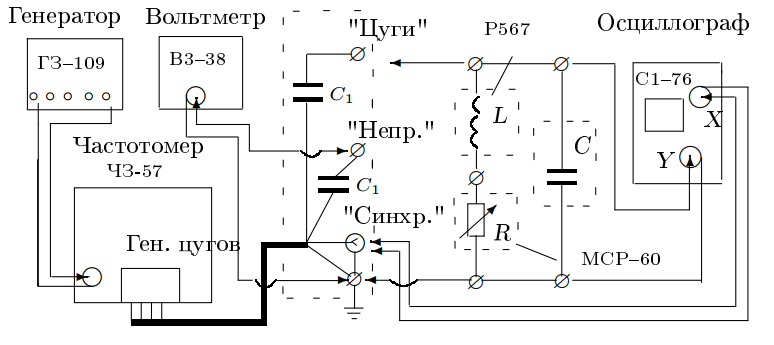
\includegraphics[width=10cm]{fig1.PNG}
    \caption{Схема экспериментальной установки для исследования вынужденных колебаний}
    \label{fig:vac}
\end{figure}

Колебательный контур состоит из ёмкости $C = 0,1$ мкФ, индуктивности $L = 100$  мГн и переменного сопротивления $R$ \par
Также учтём достаточно большое сопротивление магазина индуктивностей и уточним фактическую его индуктивность
\begin{center}
    $R_L = 30,418$ Ом \hspace{1cm} $L = 100,4$ мГн
\end{center}

Погрешность магазинов индуктивностей и сопротивлений
\begin{center}
    $\sigma_L = 0.2008\%$ \hspace{1cm} $\sigma_R = 0,02\%$
\end{center}

\section{Ход работы}
\subsection{Исследование резонансных кривых}
\begin{enumerate}
    \item Соберём цепь на рис. 1, настроим приборы. Рассчитаем резонансную частоту по формуле (1) $ \nu_0 = \frac{1}{2\pi \sqrt{LC}} = 1591,55$ Гц. Меняя частоту генератора в обе стороны от резонансной, снимем зависимость показаний вольтметра $U$ от показаний частотомера $\nu$. Результаты измерений занесём в таблицы 1 и 2.
    
        \begin{table}[h]
    \centering
    \begin{center}
    \caption{Зависимость показаний вольтметра от частоты колебаний в контуре, R = 0 Ом}
    \end{center}
    \vspace{0.1cm}
    \label{tab:my_label}
    \begin{tabular}{ |p{1.5cm}||p{0.7cm}|p{0.7cm}|p{0.7cm}|p{0.7cm}|p{0.7cm}|p{0.7cm}|p{0.7cm}|p{0.7cm}|p{0.7cm}|p{0.7cm}|p{0.7cm}|  }
 \hline
 $U$,x10 В  & 12 & 13 & 14 & 15 & 16 & 17 & 18 & 19 & 20 & 21 & 22   \\
\hline 
 $\nu$, Гц & 1484 & 1490 & 1494 & 1499 & 1503 & 1507 & 1510 & 1514 & 1516 & 1518 & 1521 \\
 \hline
 \hline
 
  $U$,x10 В  & 23 & 24 & 25 & 26 & 27 & 28 & 29 & 29,5 & 30 & 30,5 & 30,75   \\
\hline 
 $\nu$, Гц & 1523 & 1526 & 1528 & 1531 & 1534 & 1536 & 1539 & 1541 & 1543 & 1546 & 1550 \\
 \hline
 \hline
 
  $U$,x10 В  & 30,5 & 30 & 29,5 & 29 & 28,5 & 28 & 27 & 26 & 25 & 24 & 23   \\
\hline 
 $\nu$, Гц & 1551 & 1557 & 1559 & 1561 & 1563 & 1564 & 1566 & 1569 & 1572 & 1575 & 1577 \\
 \hline
 \hline
 
  $U$,x10 В  & 22 & 21 & 20 & 19 & 18 & 17 & 16 & 15 & 14 & 13 & 12   \\
\hline 
 $\nu$, Гц & 1580 & 1585 & 1587 & 1590 & 1593 & 1597 & 1602 & 1606 & 1611 & 1618 & 1624 \\

 \hline
\end{tabular}
\end{table}

        \begin{table}[h]
    \centering
    \begin{center}
    \caption{Зависимость показаний вольтметра от частоты колебаний в контуре, R = 100 Ом}
    \end{center}
    \vspace{0.1cm}
    \label{tab:my_label}
    \begin{tabular}{ |p{1.5cm}||p{0.7cm}|p{0.7cm}|p{0.7cm}|p{0.7cm}|p{0.7cm}|p{0.7cm}|p{0.7cm}|p{0.7cm}|p{0.7cm}|p{0.7cm}|p{0.7cm}|  }
 \hline
 $U$,x3 В  & 20 & 21 & 22 & 23 & 24 & 25 & 26 & 27 & 28 & 28,5 & 29   \\
\hline 
 $\nu$, Гц & 1439 & 1448 & 1457 & 1465 & 1472 & 1481 & 1489 & 1496 & 1506 & 1510 & 1515 \\
 \hline
 \hline
 
  $U$,x3 В  & 29,5 & 30 & 30,5 & 31 & 31,2 & 31 & 30,5 & 30 & 29,5 & 29 & 28,5   \\
\hline 
 $\nu$, Гц & 1521 & 1527 & 1535 & 1549 & 1558 & 1567 & 1581 & 1589 & 1596 & 1604 & 1609 \\
 \hline
 \hline
 
  $U$,x3 В  & 28 & 27 & 26 & 25 & 24 & 23 & 22 & 21 & 20   \\
\hline 
 $\nu$, Гц & 1615 & 1626 & 1637 & 1648 & 1659 & 1670 & 1682 & 1695 & 1708  \\
 \hline

\end{tabular}
\end{table}
    
    \item Построим резонансные кривые на одном графике в координатах $U/U_0 = f(\nu/\nu_0)$ (рис. 2).
    
\begin{figure}[h]
    \centering
    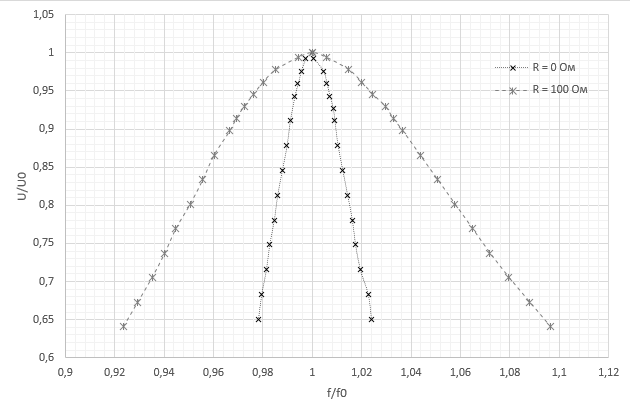
\includegraphics[width=\textwidth]{graph1.PNG}
    \caption{Резонансные кривые для цепей с сопротивлением R = 0 Ом и R = 100 Ом}
    \label{fig:vac}
\end{figure}

\item По формуле (2) определим добротность колебательного контура при разных значениях R:
\begin{center}
$Q_0 = \frac{\nu_0}{\triangle \nu_1} = \frac{1550}{38} = 26,271$ \\
$Q_{100} = \frac{\nu_0}{\triangle \nu_2} = \frac{1558}{144,4} = 6,924$
\end{center}

Погрешность измерения ширины резонансной кривой определим по методу наименьших квадратов (прямые на резонансных кривых до начала перегиба, $\approx$ 0,95 по оси y). 
$$\sigma_{\triangle \nu} = \frac{1}{\sqrt{n}} \sqrt{\frac{<y^2>-<y>^2}{<x^2>-<x>^2} - b^2}$$

Тогда для погрешности добротности формула
$$\sigma_Q = Q\sqrt{(\frac{\sigma_{\nu_0}}{\nu_0})^2 + (\frac{\sigma_{\triangle \nu}}{\triangle \nu})^2}$$

Окончательно получим

\begin{center}
$Q_0 =  26,271 \pm 0,231 \hspace{1cm} \epsilon_0 = 0,88\% $\\
$Q_{100} =  6,924 \pm 0,005 \hspace{1cm} \epsilon_0 = 0,07\% $

\end{center}

\item Определим экспериментальное значение добротности контура по формуле $Q = \frac{1}{R}\sqrt{\frac{L}{C}}$

\begin{center}
    $Q_0 = 32,93 \hspace{1cm} Q_{100} = 7,68$
\end{center}

\end{enumerate}

    
\subsection{Процессы установления и затухания колебаний}

\begin{enumerate}
    \item Подключим контур к клемме "Цуги". Установим на генераторе резонансную частоту, подберём частоту развёртки ЭО, при которой на экране укладывается один цуг колебаний. Рассчитаем добротность контура при нарастании и затухании колебаний, пользуясь формулами (3) и (4). Результаты измерения запишем в таблицы 3 - 6. Фотографии картинки на осциллографие при нарастании и затухании колебаний при разных сопротивлениях в цепи представлены на рис. 3 и 4.
    
    $$ Q_{up} = \frac{\pi}{\Theta} =  \pi (\frac{1}{n} ln \frac{U_0 - U_k}{U_0 - U_{k+n}})^-^1 $$

$$ Q_{down} = \frac{\pi}{\Theta} = \pi (\frac{1}{n} ln \frac{U_k}{U_{k+n}})^-^1 $$
    
        \begin{table}[h]
    \centering
    \begin{center}
    \caption{Нарастание колебаний, R = 0 Ом}
    \end{center}
    \vspace{0.1cm}
    \label{tab:my_label}
    \begin{tabular}{ |p{1.5cm}|p{1.5cm}|p{1.5cm}|p{1.5cm}|p{1.5cm}|p{1.5cm}|p{1.5cm}|p{1.5cm}|p{1.5cm}|p{1.5cm}|p{1.5cm}|p{1.5cm}| }
 \hline
    U, дел & U_1 = 0,5 & U_2 = 1 & U_3 = 1,4 & U_4 = 1,8 & U_5 = 2,2 & U_6 = 2,5 & U_7 = 2,6 & U_8 = 2,9 & U_0 = 3,4 \\
\hline 
    Q &	15,84 & 15,49 &	12,81 &	10,91 &	10,80 &	15,49 &	10,76 &	6,40 &	6,80\\
 \hline
\end{tabular}
\end{table}

    \begin{table}[h]
    \centering
    \begin{center}
    \caption{Затухание колебаний, R = 0 Ом}
    \end{center}
    \vspace{0.1cm}
    \label{tab:my_label}
    \begin{tabular}{ |p{1.5cm}|p{1.5cm}|p{1.5cm}|p{1.5cm}|p{1.5cm}|p{1.5cm}|p{1.5cm}|p{1.5cm}|p{1.5cm}|p{1.5cm}|p{1.5cm}|p{1.5cm}| }
 \hline
    U, дел & U_1 = 2,7 & U_2 = 2,5 & U_3 = 2,2 & U_4 = 1,8 & U_5 = 1,6 & U_6 = 1,4 & U_7 = 1,3 & U_8 = 1,2 & U_9 = 1,1 \\
\hline 
    Q &	40,80 &	30,66 &	28,14 &	28,14 &	31,30 &	29,84 &	28,14 &	30,73 &	32,74\\
 \hline
\end{tabular}
\end{table}
    
    \begin{table}[h]
    \centering
    \begin{center}
    \caption{Нарастание колебаний, R = 100 Ом}
    \end{center}
    \vspace{0.1cm}
    \label{tab:my_label}
    \begin{tabular}{ |p{1.5cm}|p{1.5cm}|p{1.5cm}|p{1.5cm}|p{1.5cm}|p{1.5cm}|p{1.5cm}|p{1.5cm}|p{1.5cm}| }
 \hline
    U, дел & U_0 = 2,7 & U_1 = 0,8 & U_2 = 1,5 & U_3 = 2 & U_4 = 2,3 & U_5 = 2,5 \\
\hline 
    Q &  6,83  & 6,29  & 5,58 &	5,83 &  5,72 &	5,26 & 5,61 & 5,01\\
 \hline
\end{tabular}
\end{table}

    \begin{table}[h]
    \centering
    \begin{center}
    \caption{Затухание колебаний, R = 100 Ом}
    \vspace{0.1cm}
    \end{center}
    \label{tab:my_label}
    \begin{tabular}{ |p{1.5cm}|p{1.5cm}|p{1.5cm}|p{1.5cm}|p{1.5cm}|p{1.5cm}|p{1.5cm}|p{1.5cm}|p{1.5cm}| }
 \hline
    U, дел & U_1 = 2,3 & U_2 = 1,5 & U_3 = 1 & U_4 = 0,7 & U_5 = 0,5 & U_6 = 0,3 \\
\hline 
    Q & 7,35 &	7,54 &	7,92 &	8,23 &	7,74 &	8,24 &	8,57 &	7,80\\
 \hline
\end{tabular}
\end{table}

Рассчитаем погрешность определения средней величины Q по формуле $$\sigma_Q = \sqrt{\frac{1}{n(n-1)}\sum(x_i - <x>)}$$

Тогда получившиеся значения добротностей для каждой серии измерений:

\begin{center}
 
    $Q_0_u_p = 12,189 \pm 12,891$ \hspace{1cm}  $\epsilon = 105,8\% $ \\
    $Q_0_d_o_w_n = 30,403 \pm 38,634$  \hspace{1cm} $\epsilon = 127,1\% $\\
    $Q_{100 up} = 5,766 \pm 1,169$ \hspace{1cm}  $ \epsilon = 20,3\% $ \\
    $Q_{100 down} = 7,925 \pm 1,133$ \hspace{1cm}  $\epsilon = 14,3\% $
    
\end{center}

\newpage

\begin{figure}[b]
   \caption{Биения при R = 0 Ом и R = 100 Ом}
\begin{minipage}[h]{0.49\linewidth}
\center{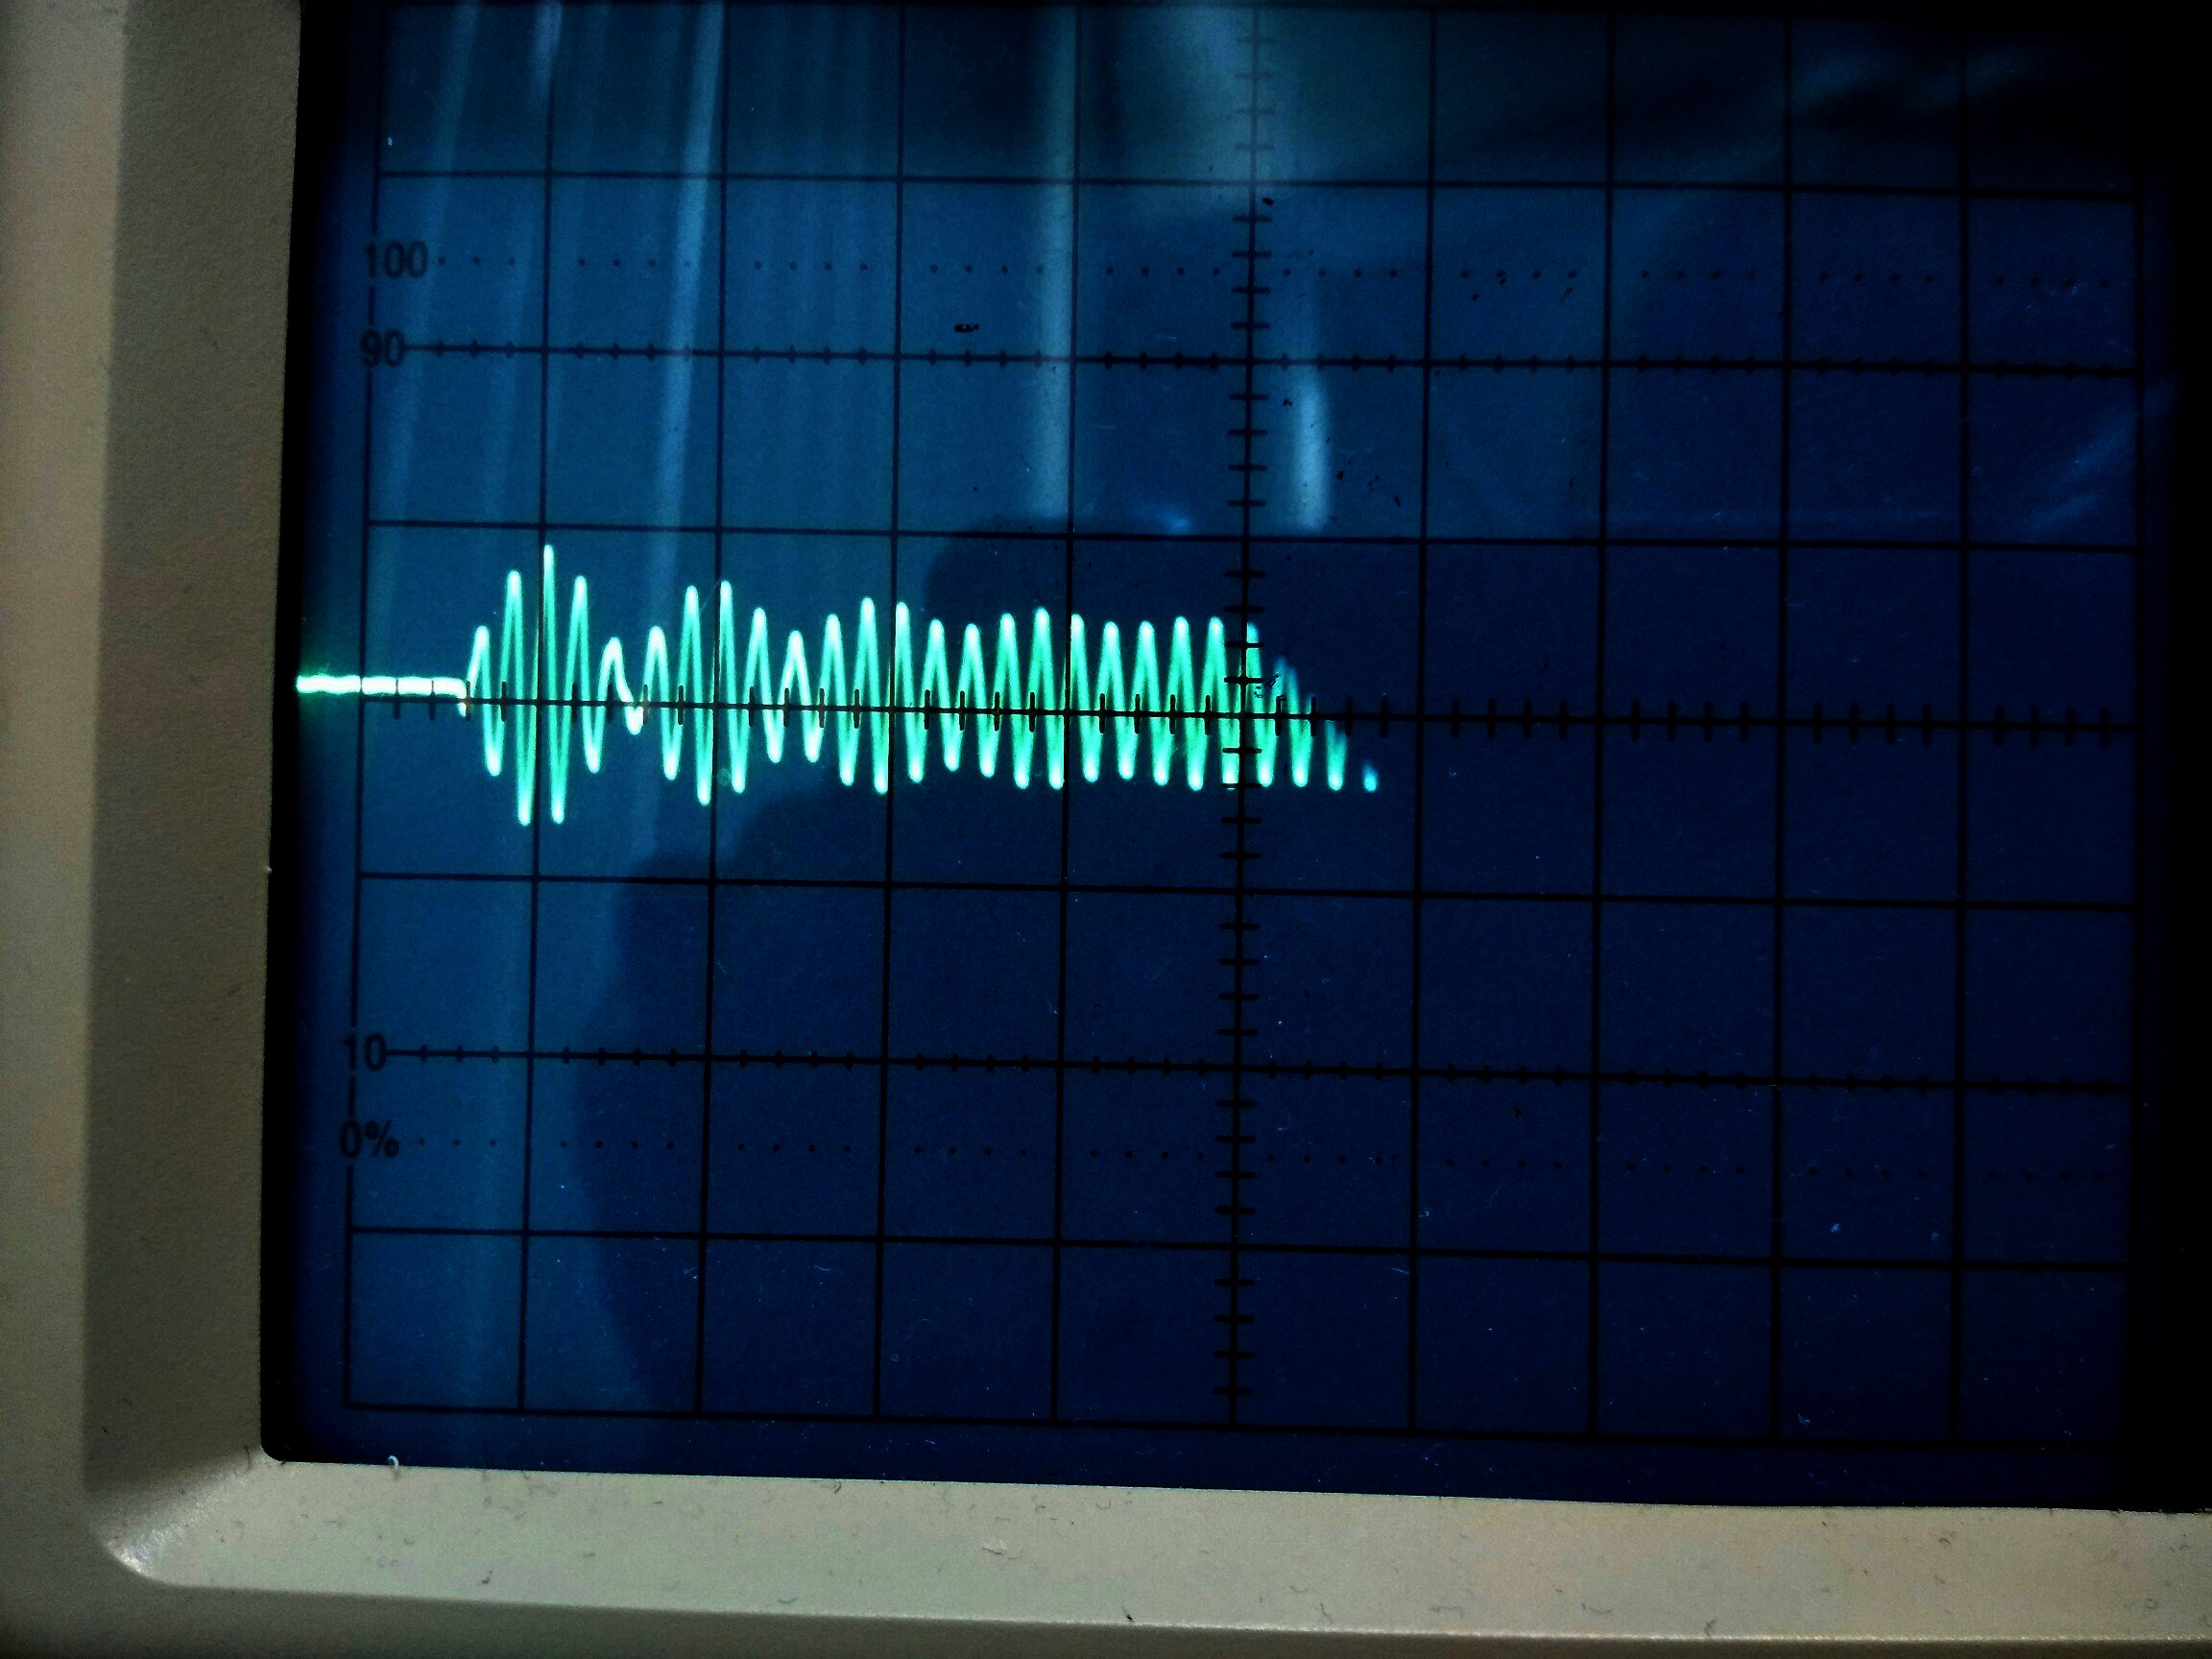
\includegraphics[width=\linewidth]{beat_0.jpg}}
\end{minipage}
\begin{minipage}[h]{0.49\linewidth}
\center{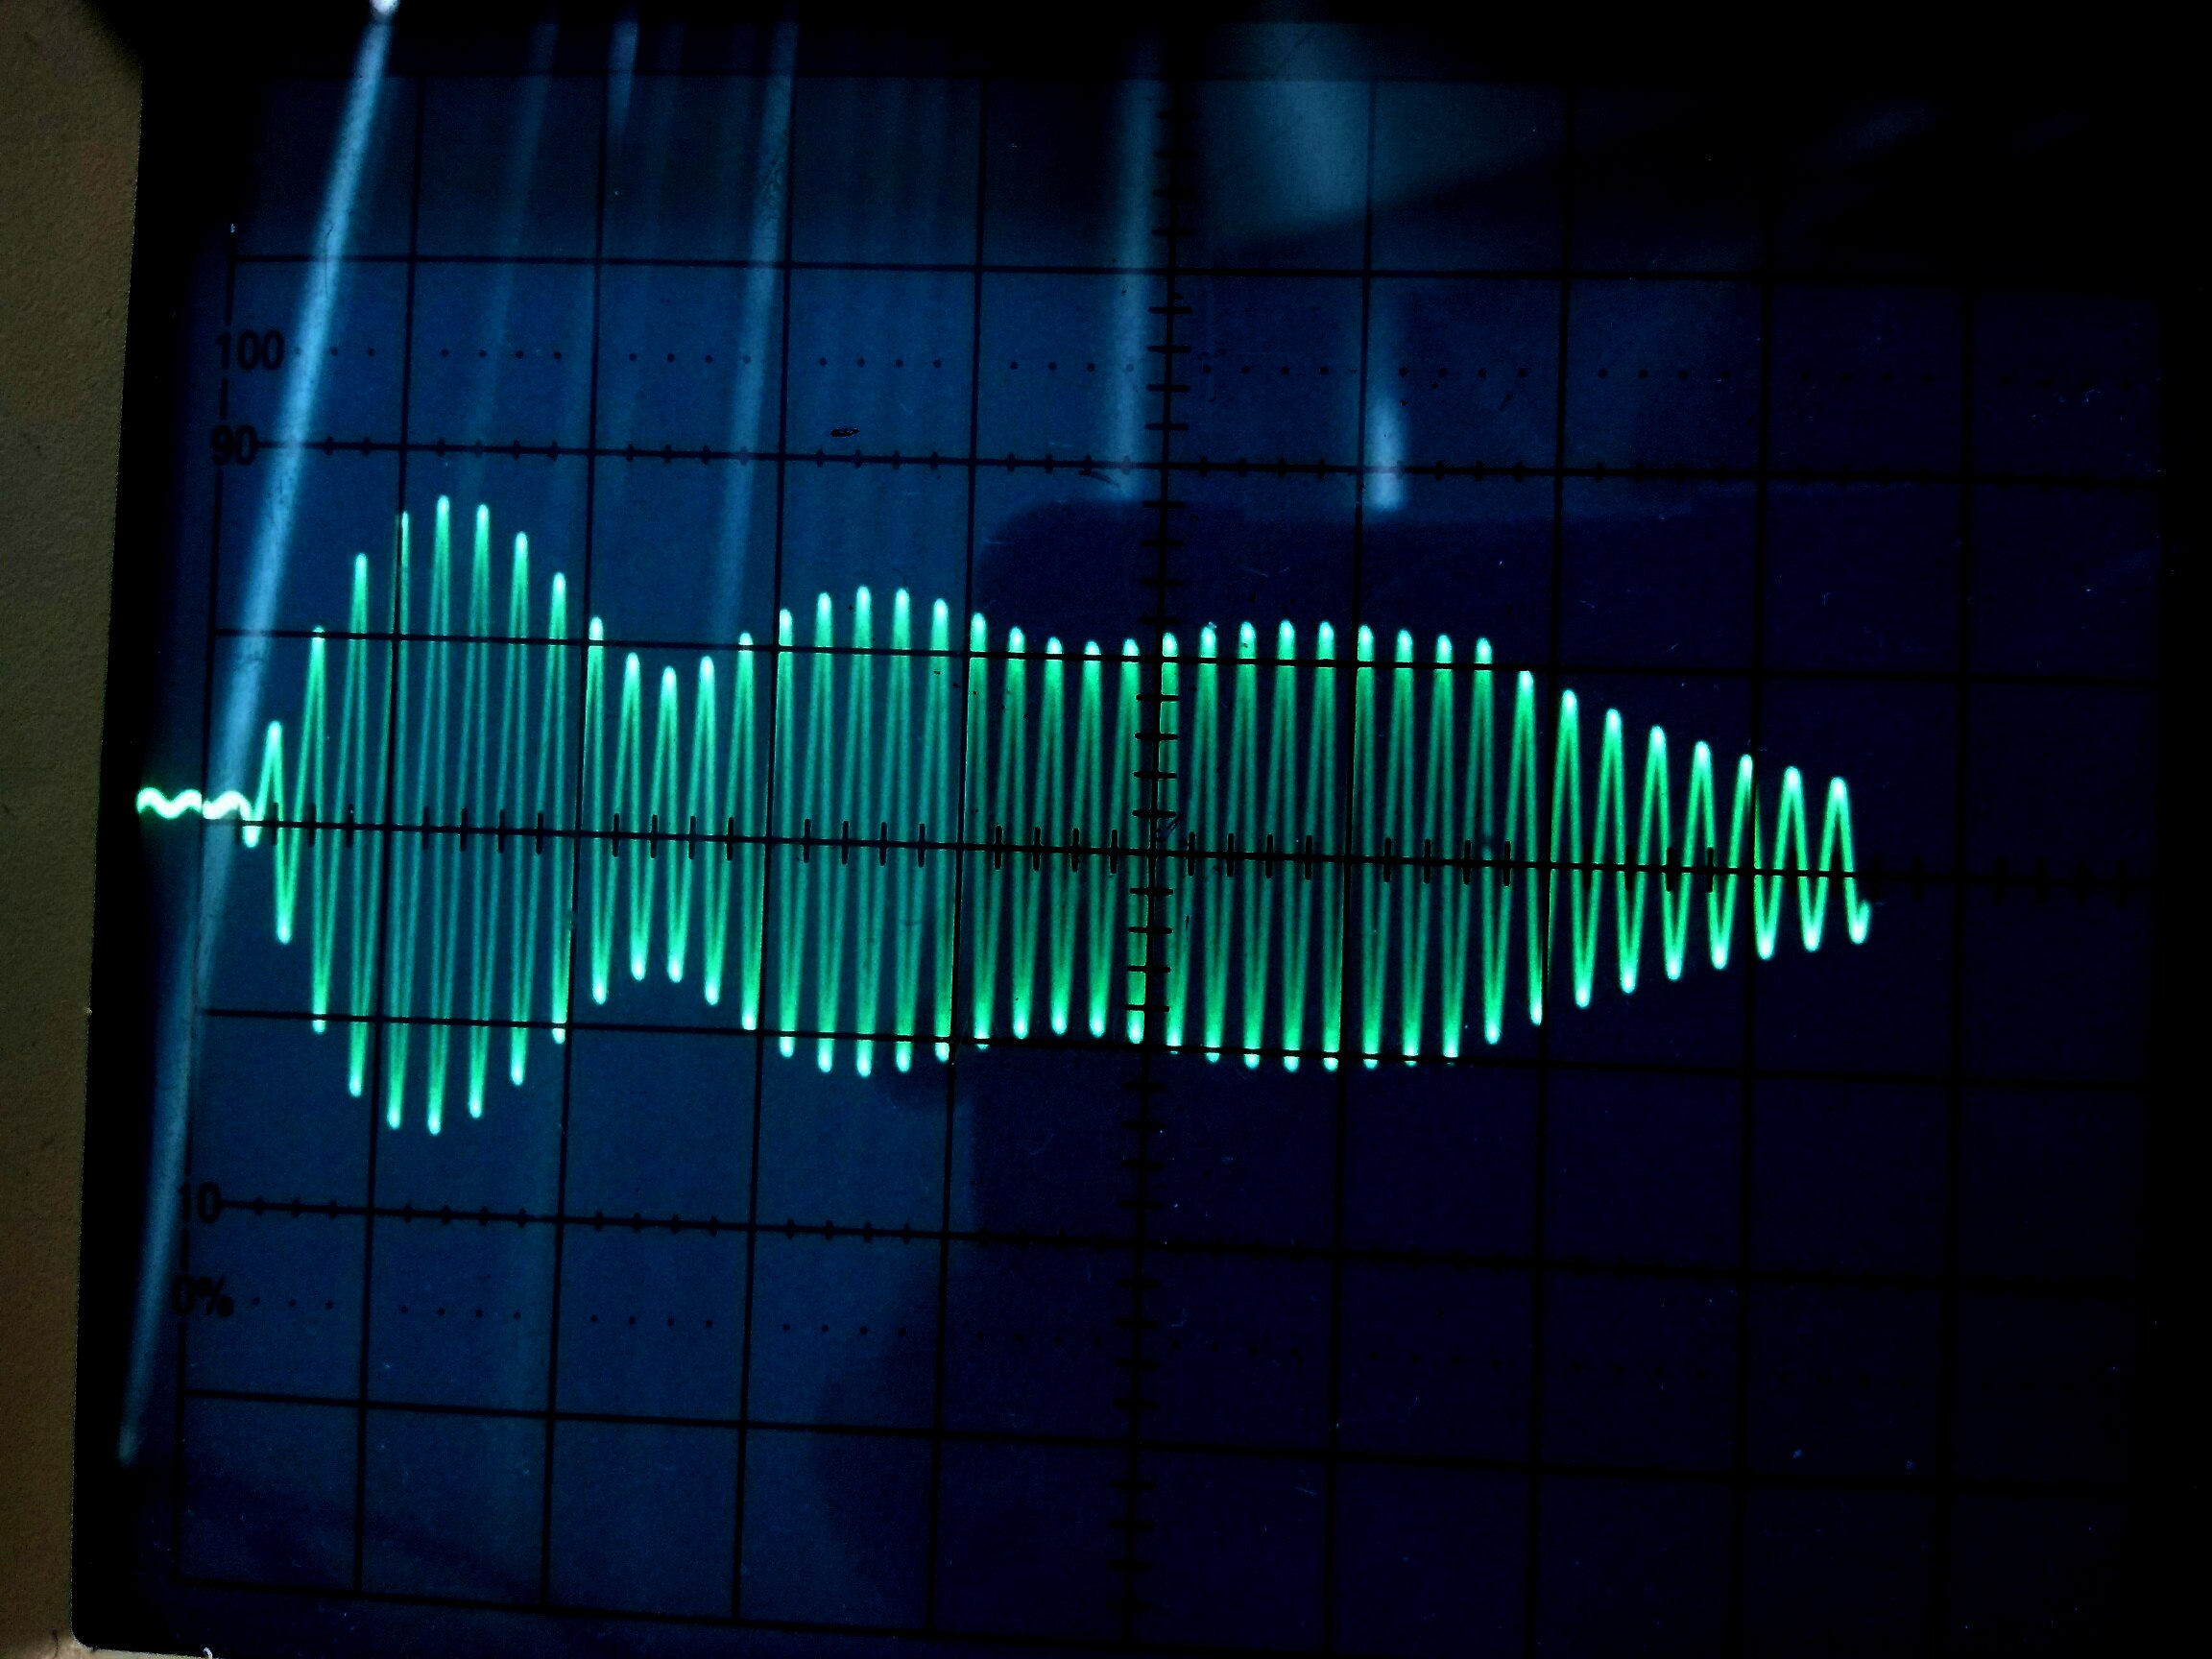
\includegraphics[width=\linewidth]{beat_100.jpg}}
\end{minipage}
\label{ris:image1}
\end{figure}

\item Сместим частоту генератора с резонансного значения и получим на экране картину биений (см. рис 5). Они возникают из-за того, что частота близка к резонансной и разность фаз колебаний на частоте генератора и на резонансной частоте меняется медленно. Когда экспонента $e^{-\frac{\omega_0}{2Q}t}$ достаточно затухнет, колебания станут синусоидальными

\item Сведём результаты всех измерений в таблицу 7

    \begin{table}[h]
    \centering
    \begin{center}
    \caption{Результаты измерений разными методами}
    \end{center}
    \vspace{0.1cm}
    \label{tab:my_label}
    \begin{tabular}{ |p{2cm}|p{2cm}||p{2cm}|p{2cm}|p{2cm}|p{2cm}| }
 \hline
   R, Ом & R_{real}, Ом & Кривая & Нарастание & Затухание & Теория\\
\hline 
 \hline
  0 & 30,428 & 26,271 & 12,19 & 30,40 & 32,93\\
 \hline
 100 & 130,428 & 6,924 & 5,77 & 7,92 & 7,68\\
 \hline
\end{tabular}
\end{table}
\begin{figure}[h]
   \caption{Нарастание и затухание колебаний при R = 0 Ом}
\begin{minipage}[h]{0.49\linewidth}
\center{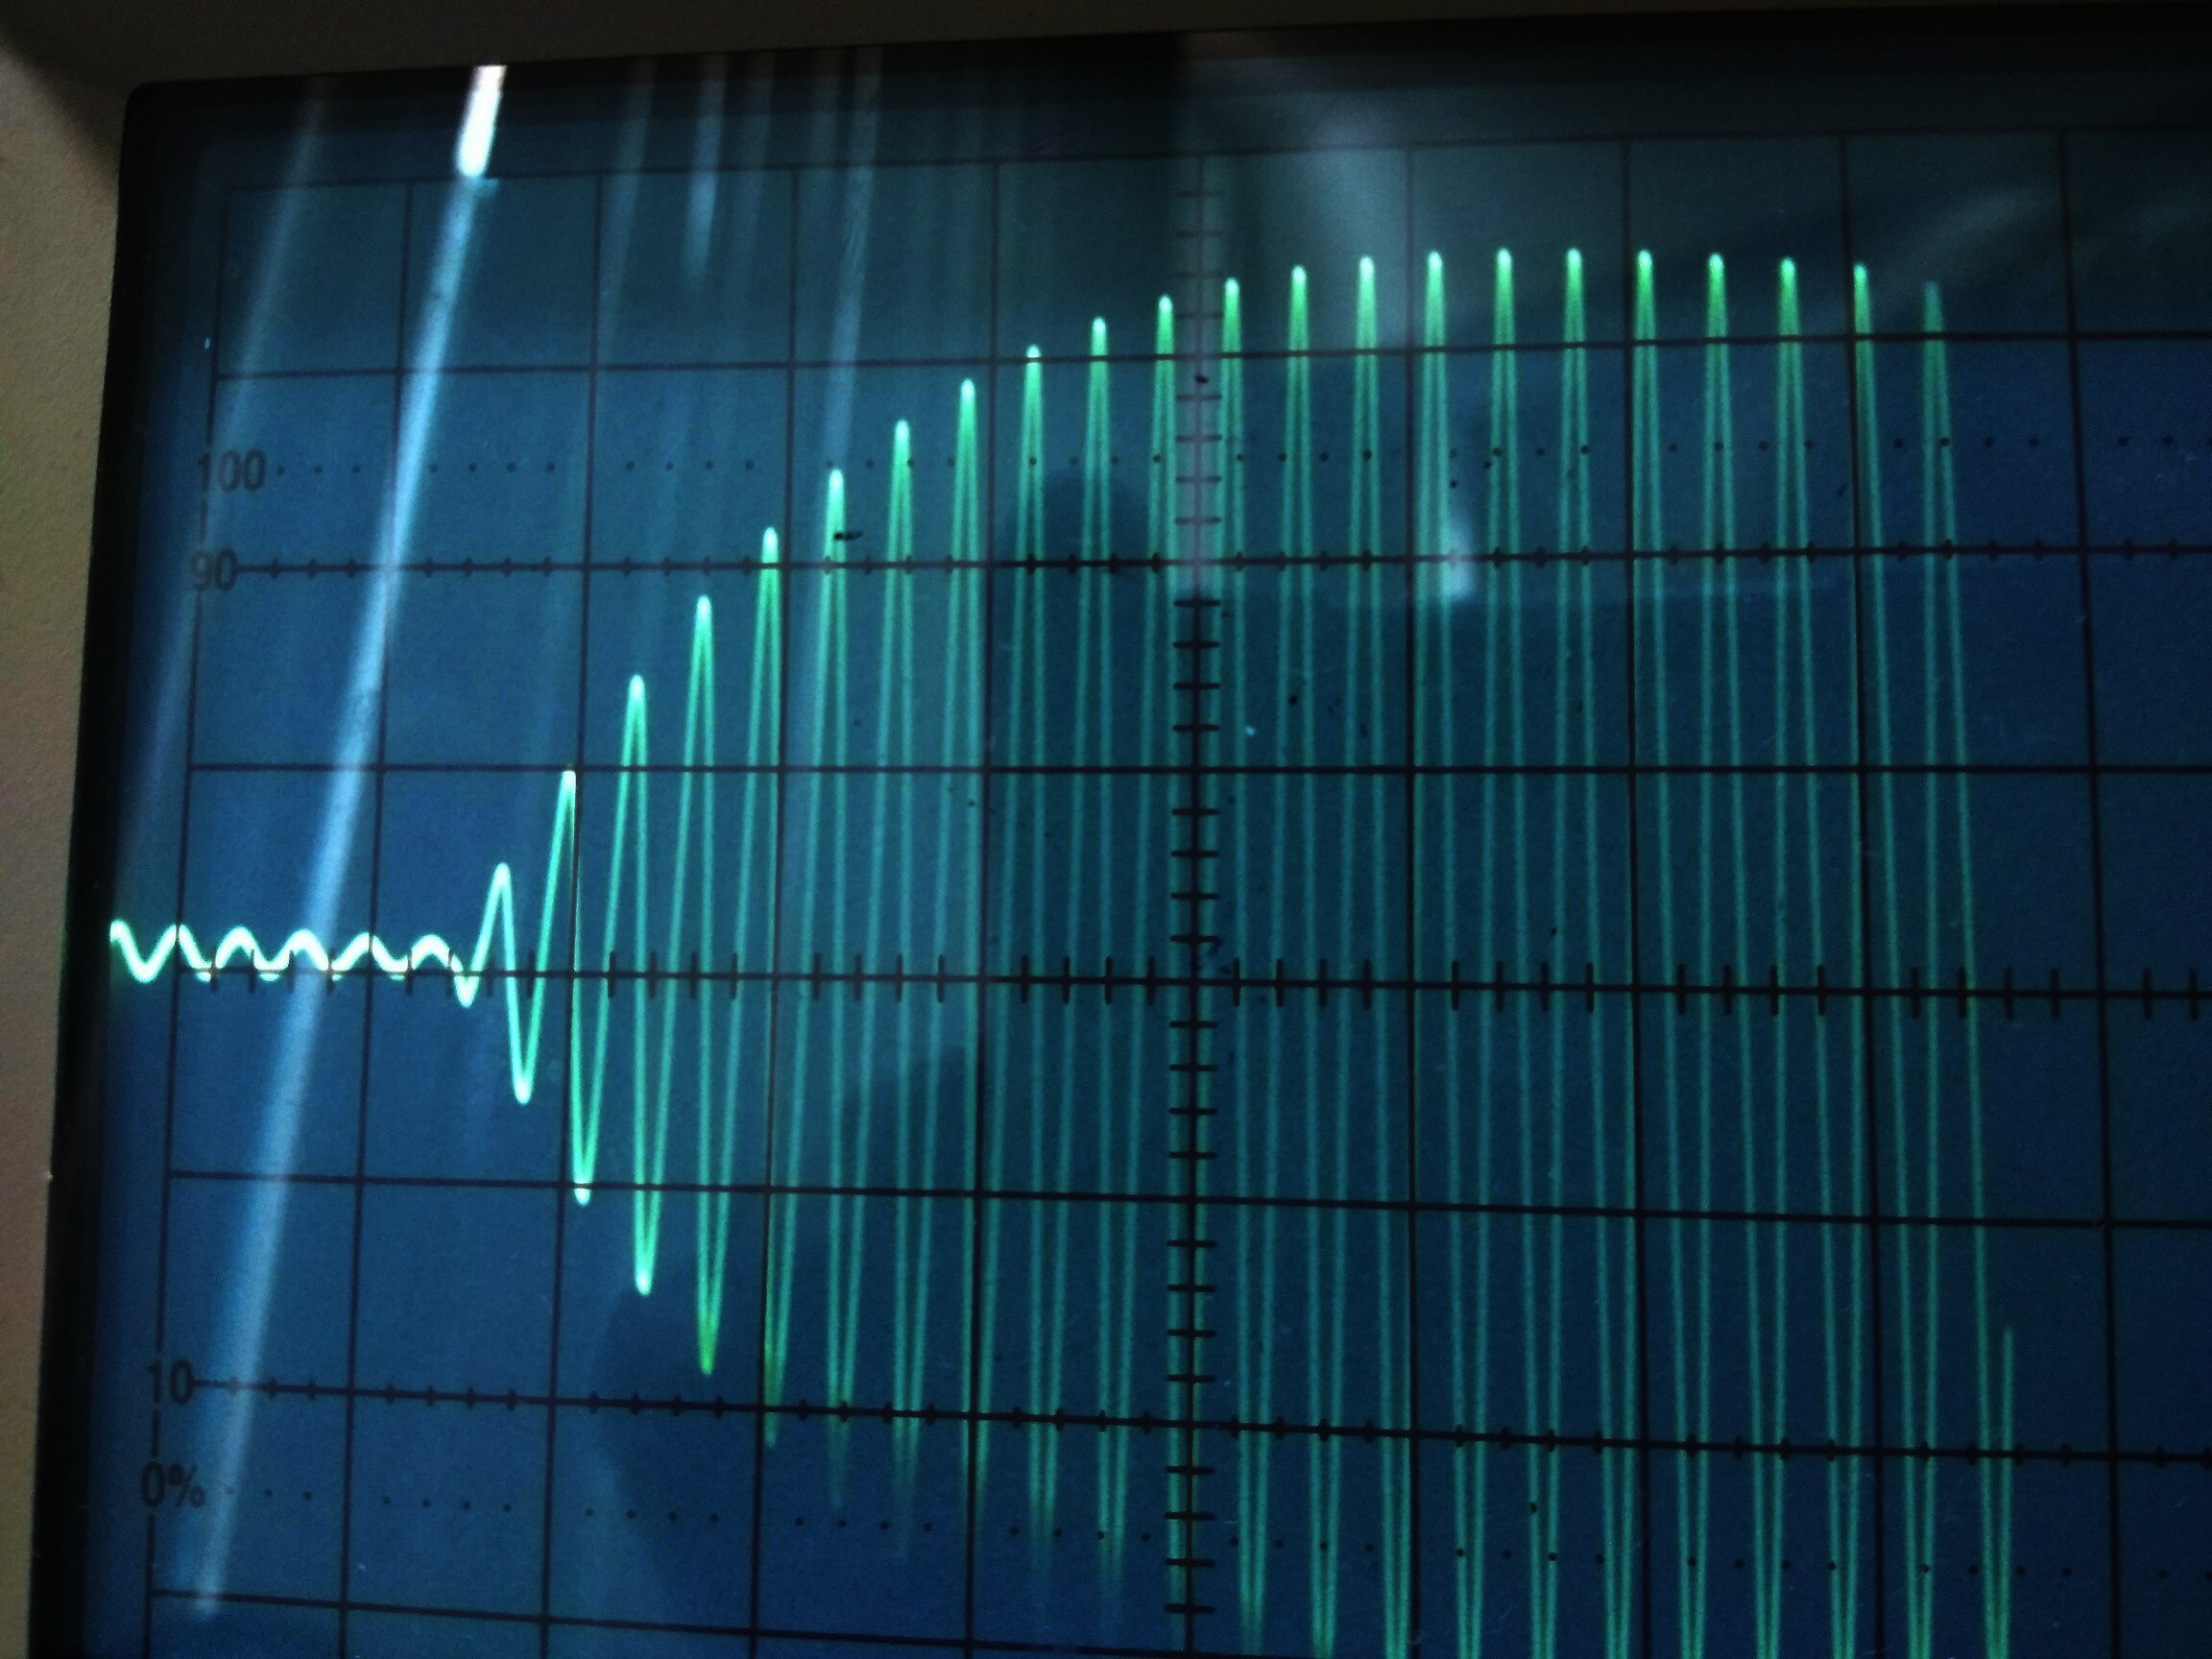
\includegraphics[width=\linewidth]{up_100.jpg}}
\end{minipage}
\begin{minipage}[h]{0.49\linewidth}
\center{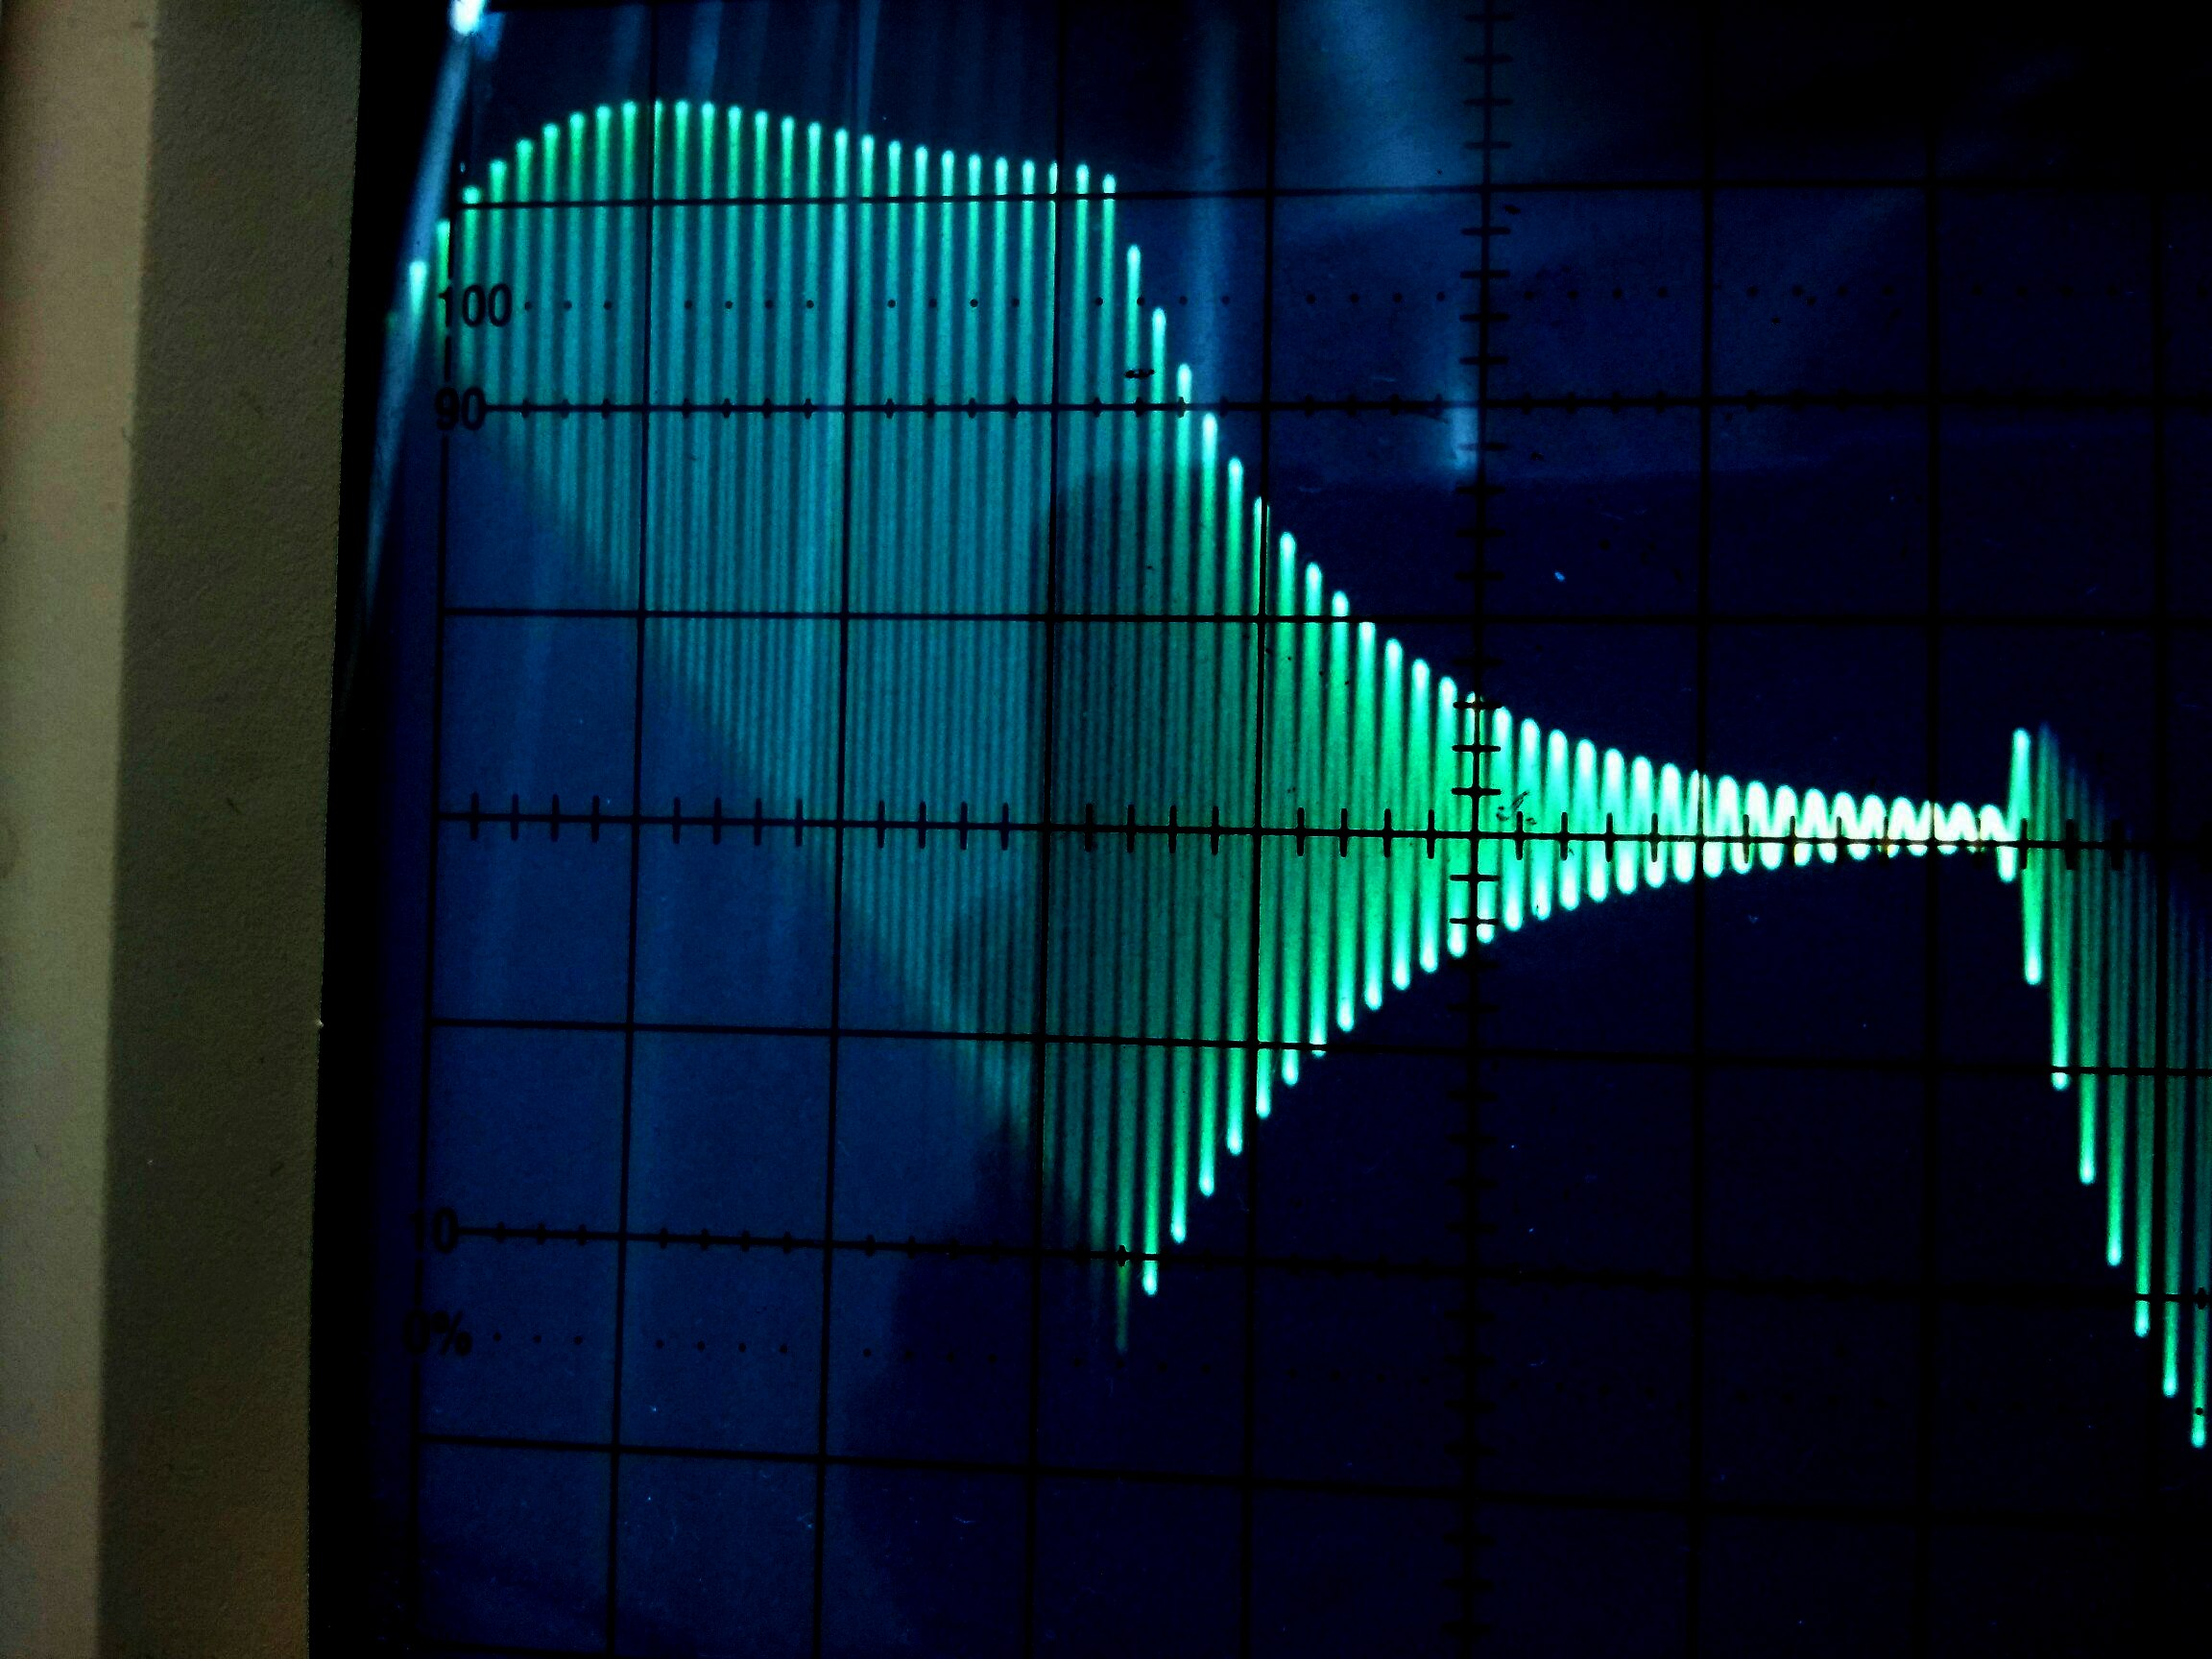
\includegraphics[width=\linewidth]{down_100.jpg}}
\end{minipage}
\label{ris:image1}
\end{figure}

\begin{figure}[h]
   \caption{Нарастание и затухание колебаний при R = 100 Ом}
\begin{minipage}[h]{0.49\linewidth}
\center{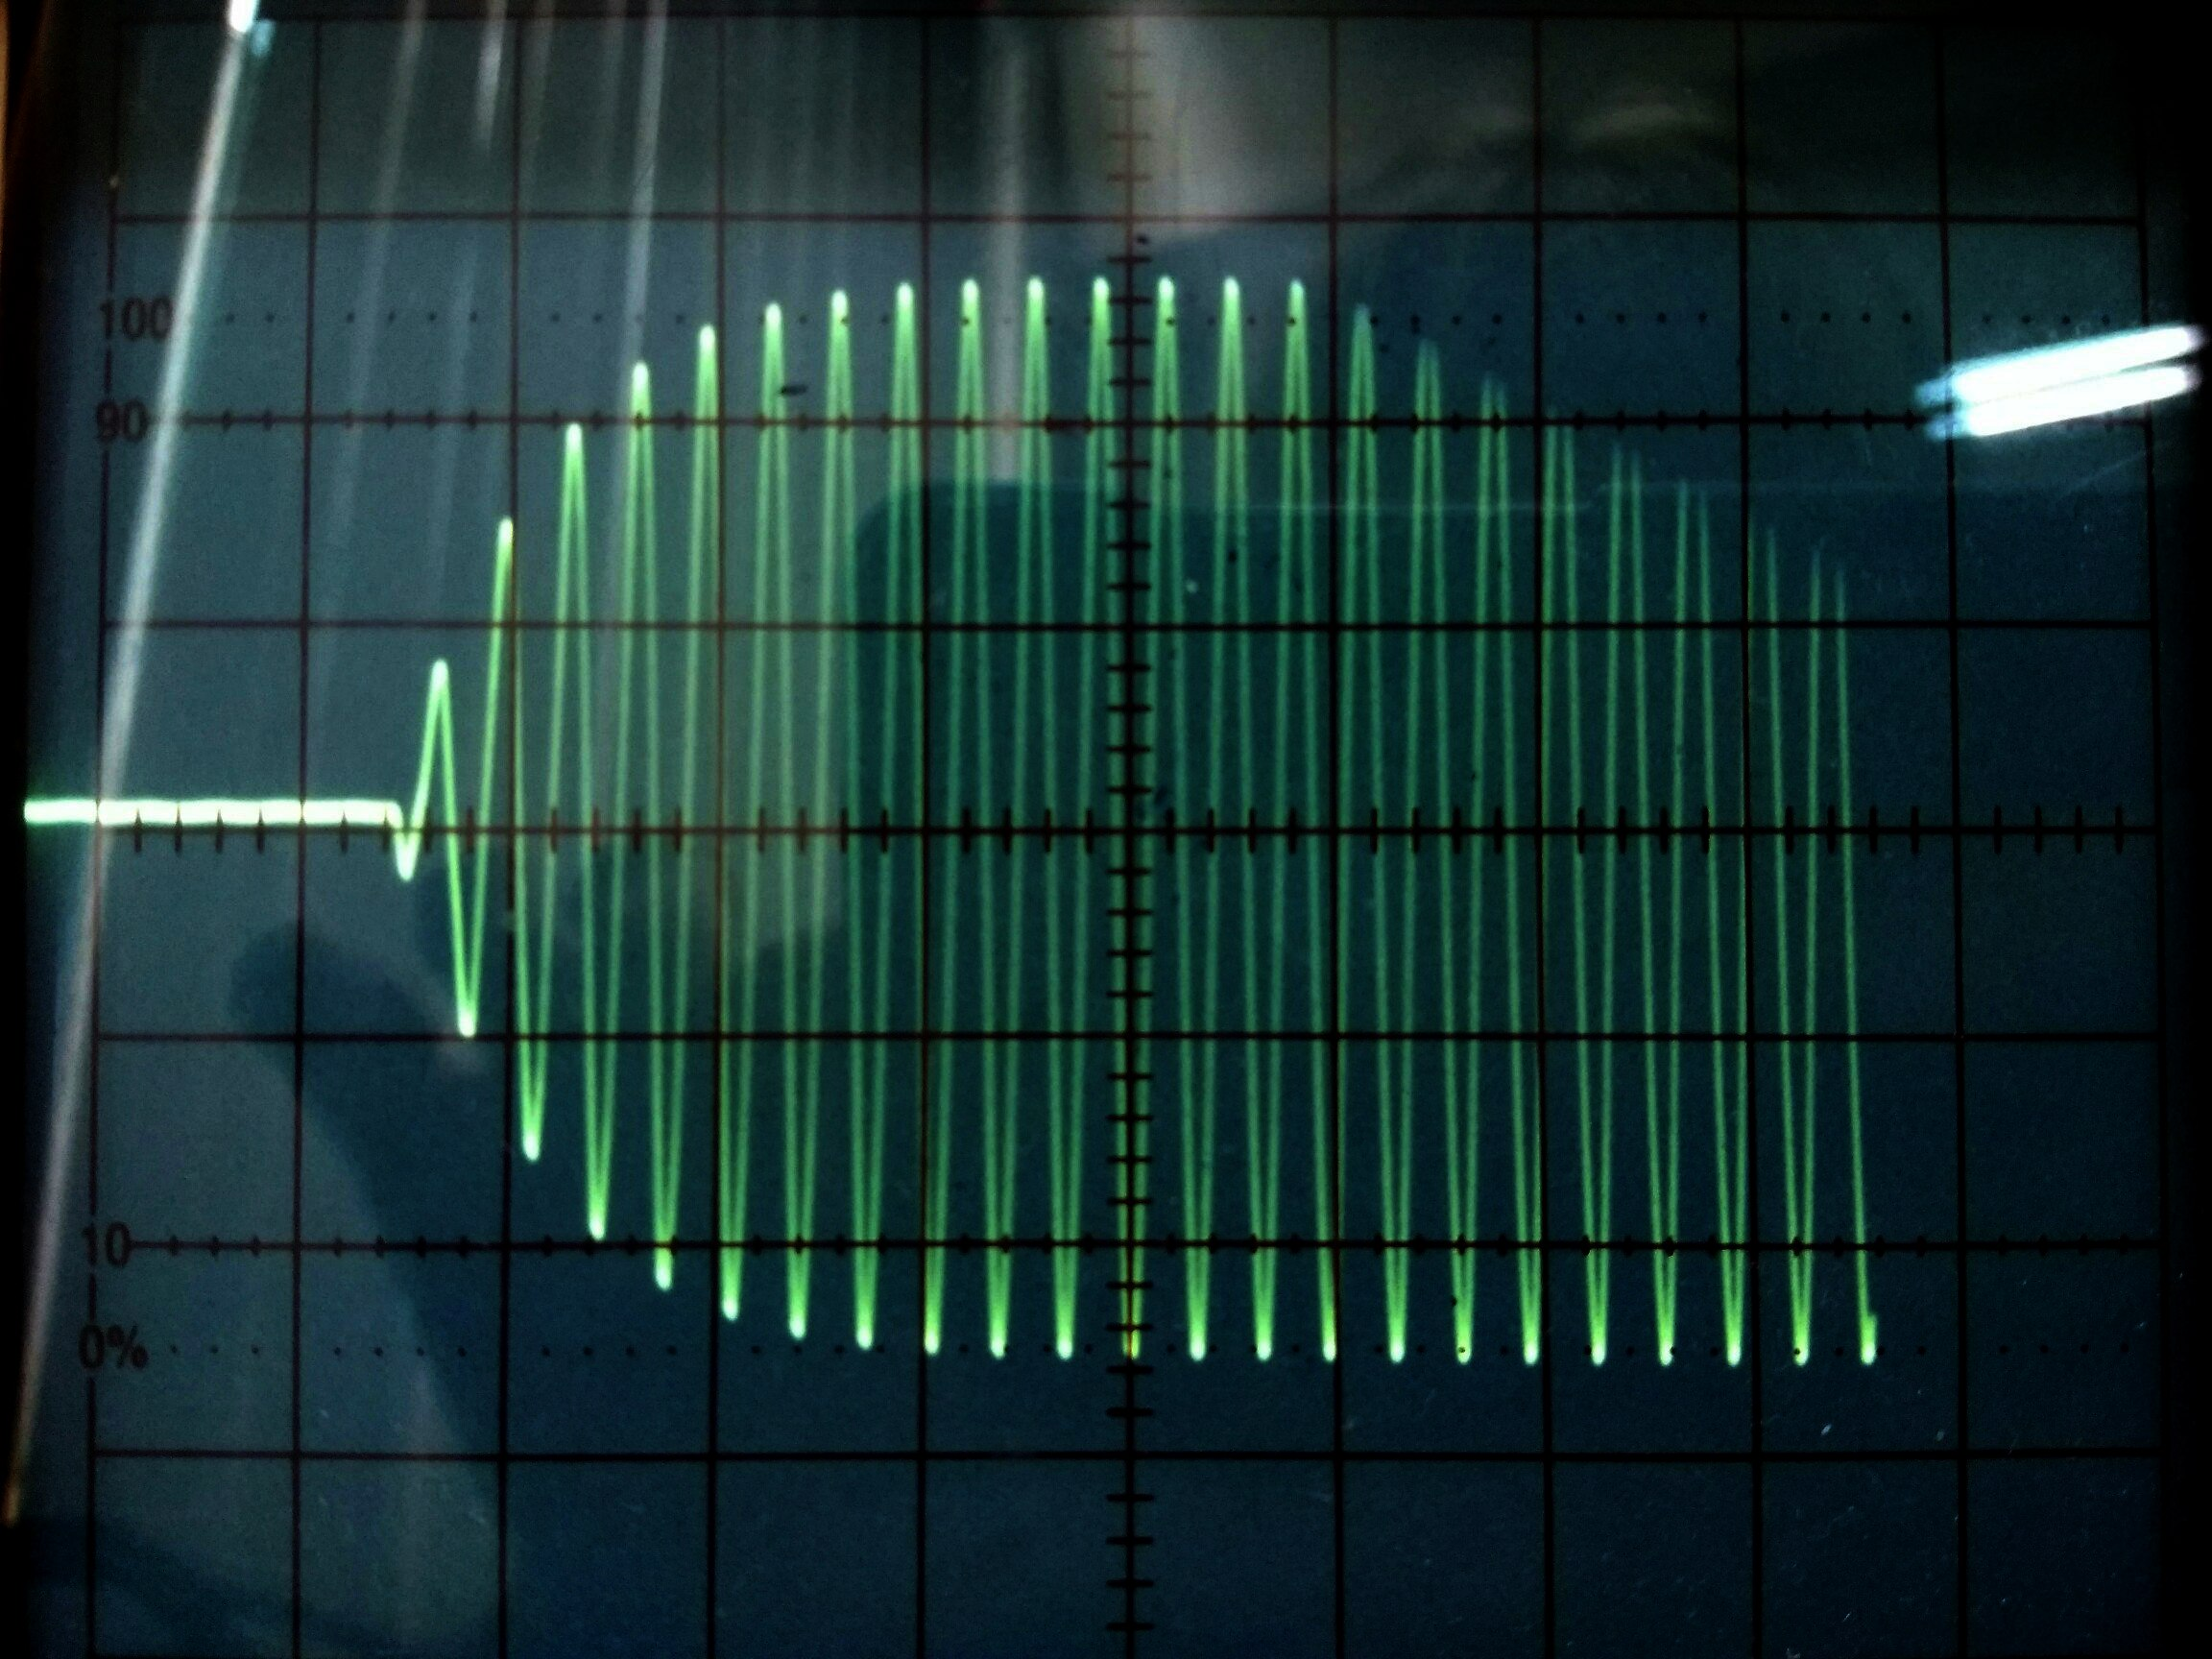
\includegraphics[width=\linewidth]{up_0.jpg}}
\end{minipage}
\begin{minipage}[h]{0.49\linewidth}
\center{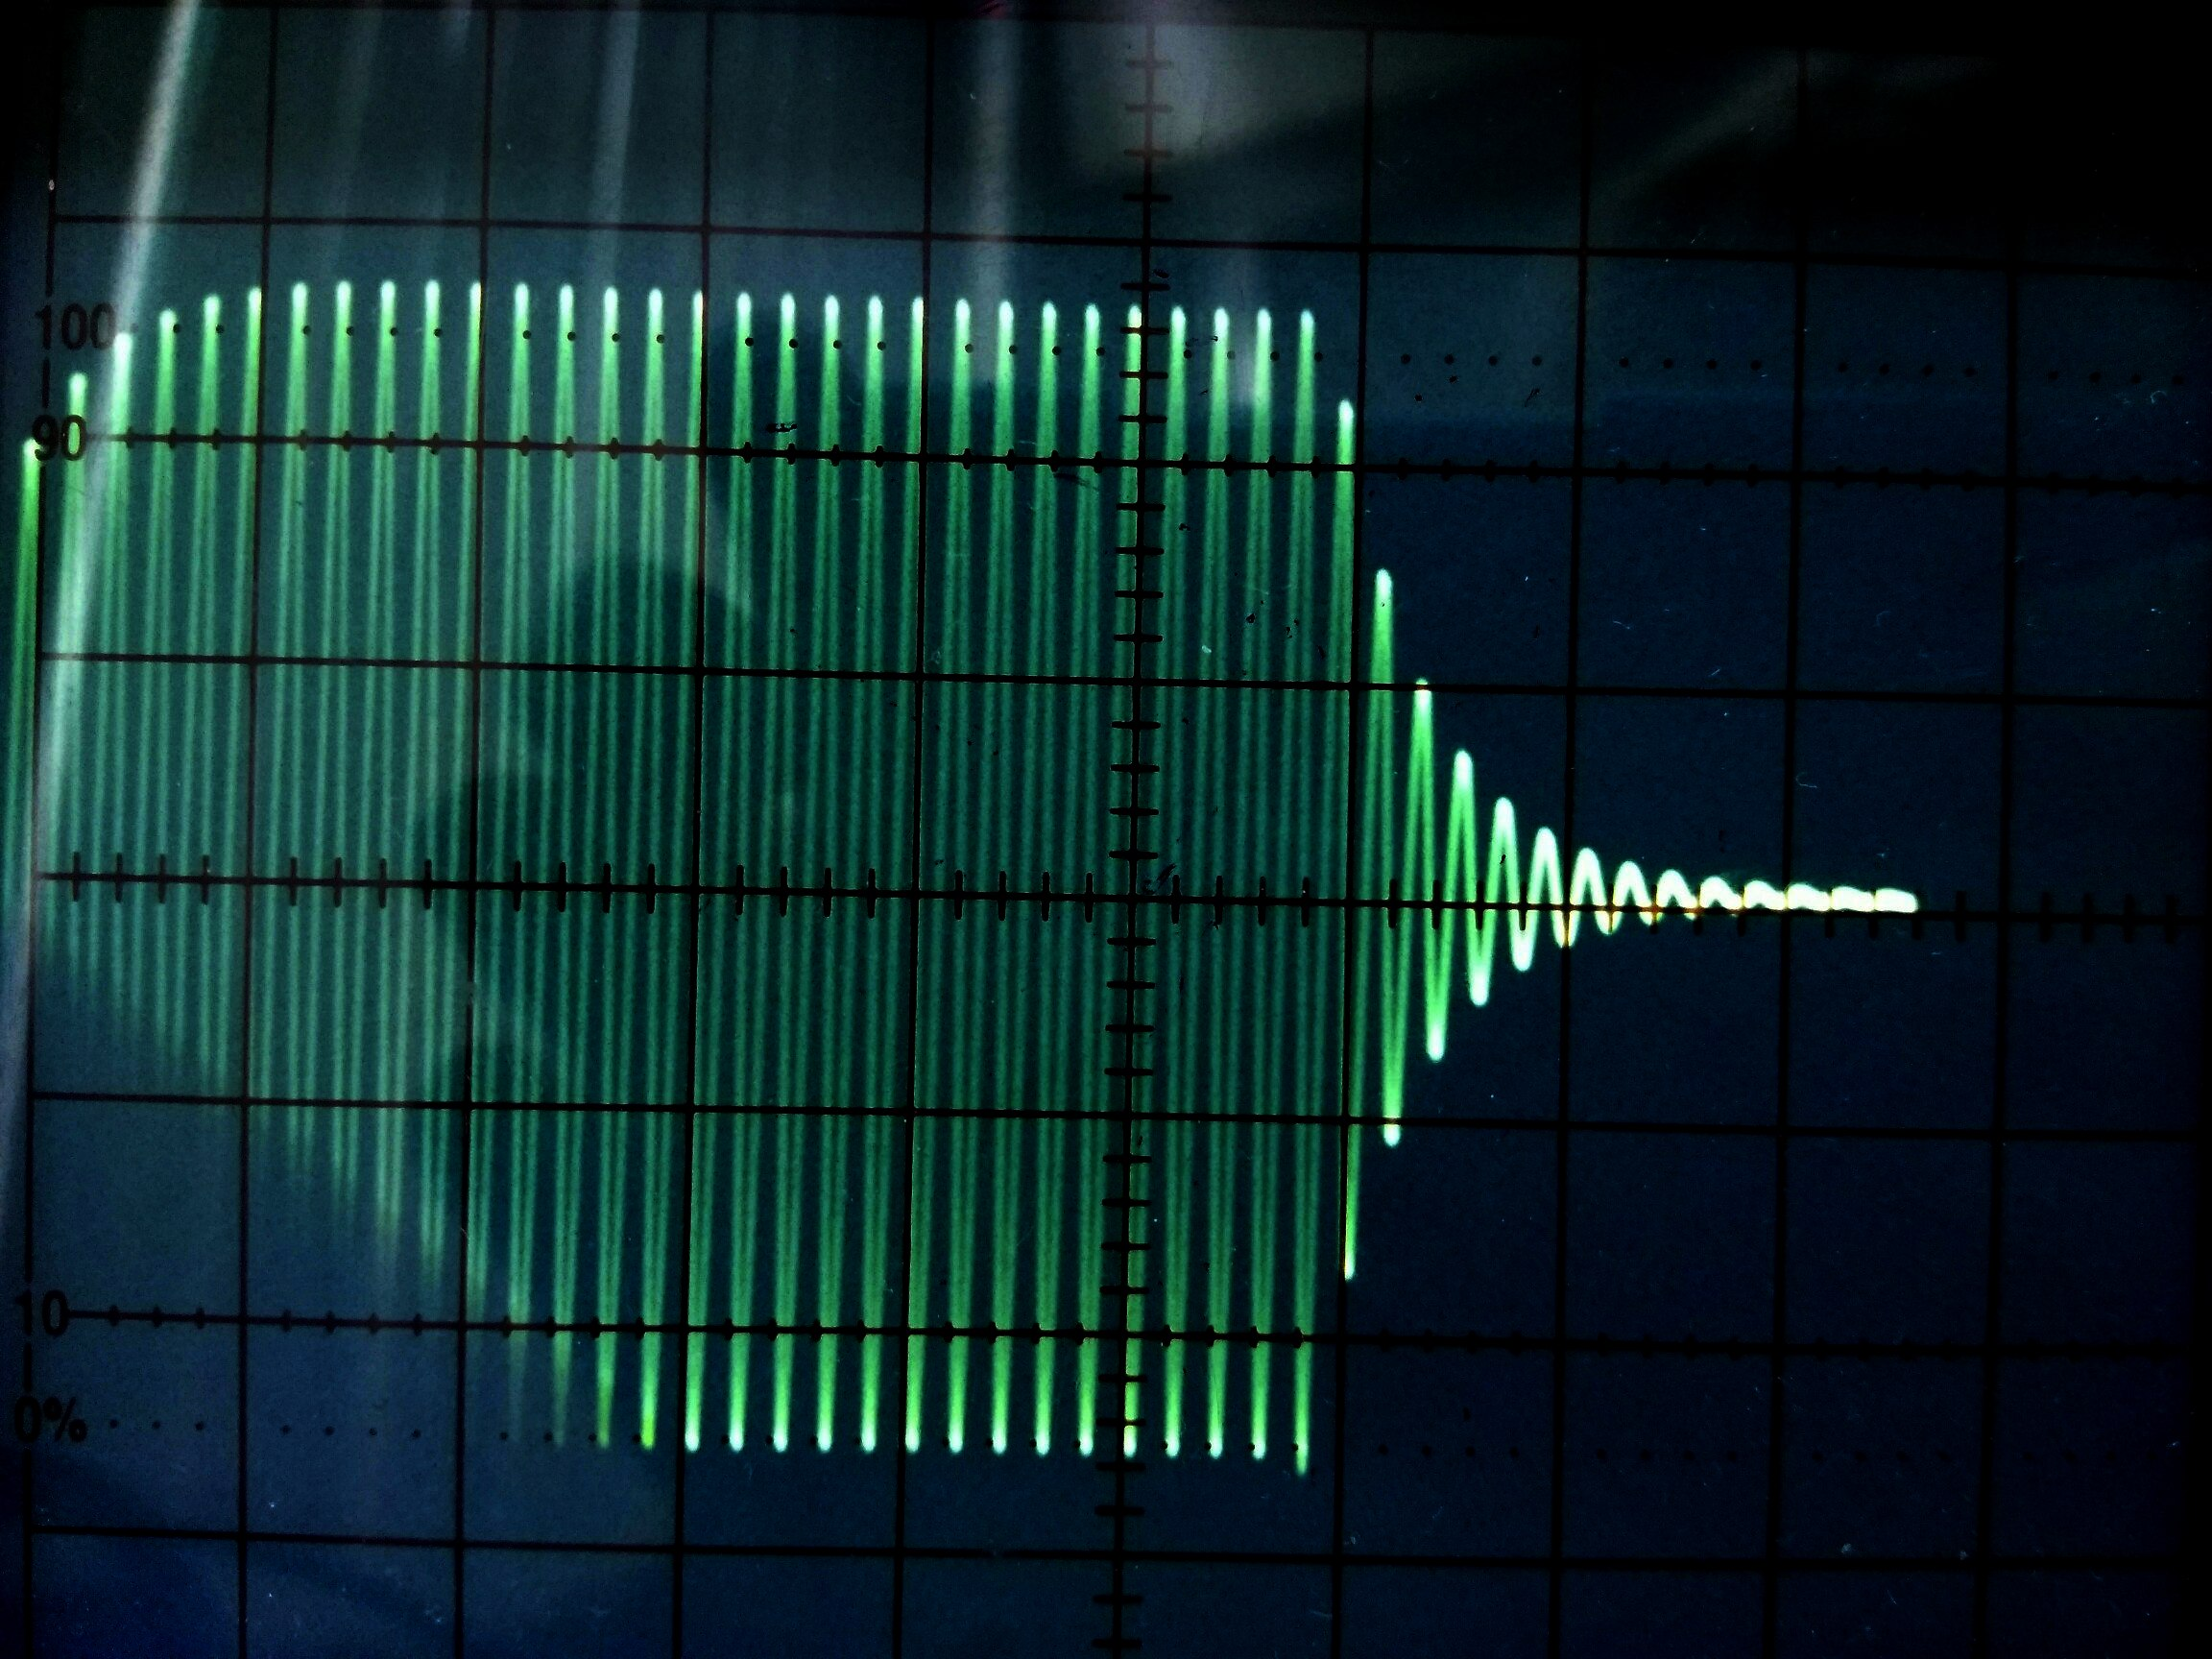
\includegraphics[width=\linewidth]{down_0.jpg}}
\end{minipage}
\label{ris:image1}
\end{figure}


\end{enumerate}

\newpage
\section{Вывод}
В ходе работы были изучены процессы вынужденных колебаний в электрическом контуре. Были исследованы резонансные кривые для двух контуров с разными сопротивлениями, найдена добротность этих контуров по полученным кривым. Также добротность была найдена при изучении установления колебаний в контуре при запуске в него цугов волн - при нарастании и затухании колебаний. Было рассчитано также теоретическое значение добротности контуров. В конце работы были сравнены все 4 значения. \par
Рассмотрим причины, почему могли не сойтись значения, полученные теоретически и экспериментально. 
\begin{itemize}
    \item Наиболее вероятная причина - наличие в контуре дополнительных сопротивлений, ёмкостей и индуктивностей. Самый точный результат определения добротности - по методу резонансных кривых, и значения полученные этим методом, практически совпадают с теоретическими. Стоило с помощью LRC-моста проверить все соединения, составить более точную схему установки и работать с ней
    \item Естественно, что значения добротности контуров, полученные при исследовании нарастания и затухания цугов колебаний, плохо сходятся с теоретическими. Разброс получившихся значений очень велик, при R = 0 относительная погрешность вообще составляет больше 100\%, что говорит о некорректности эксперимента. Тем не менее, при выполнении этого задания мы посмотрели детально на процесс установления колебаний в контуре (использовать этот метод при определении добротности контура не рекомендуется)
\end{itemize}

\end{document}
